\documentclass[runningheads]{llncs}

% ---------------------------------------------------------------------------
% ATIS 2026 CAMERA-READY (paper 452) -- Track 3: Artificial Intelligence, Data
% Security and Cybersecurity. Springer CCIS format (LNCS class), <= 12 pages.
% \anonfalse (default) = named camera-ready build; \anontrue = anonymized build.
% Table bodies in tables/*.tex are generated by `python -m ffs.experiments.tables_cr`.
% ---------------------------------------------------------------------------

\usepackage[T1]{fontenc}
\usepackage{lmodern}   % Type 1 outline fonts (T1 without it embeds bitmap Type 3)
\usepackage{graphicx}
\usepackage{booktabs}
\usepackage{amsmath}
\usepackage{amssymb}
\usepackage{mathtools}
\usepackage{xcolor}
\usepackage[hidelinks]{hyperref}

% Absorb a few unavoidable wide lines without visible stretching.
\emergencystretch=2em

% Author-block toggle: \anontrue = anonymized (double-blind SUBMISSION version),
% \anonfalse = named (CAMERA-READY / records version). ATIS review appears to be
% double-blind -- flip to \anontrue before uploading the submission PDF to CMT.
\newif\ifanon
\anonfalse

% Primitive \input, so generated table bodies with \midrule work inside tabular.
\makeatletter\newcommand{\tabinput}[1]{\@@input #1 }\makeatother
\newcommand{\gprime}{g'(c)}
\newcommand{\RR}{R}
\newcommand{\RStar}{R^{\star}}

\begin{document}

\title{Knowing When to Walk Away: Foraging-Based
Frontier Scheduling for Parallel Autonomous
Penetration-Testing Agents}

\titlerunning{Foraging-Based Frontier Scheduling for Pentest Agents}

\ifanon
  \author{Anonymous Author(s)}
  \authorrunning{Anonymous}
  \institute{Affiliation withheld for double-blind review}
\else
  \author{Manas M. N. \and Chhavi Pareek \and Hitarth Mehra\thanks{Corresponding author:
    \email{hitarthmehra.cs23@rvce.edu.in}} \and Chetan M. Patil}
  \authorrunning{Manas M. N. et al.}
  \institute{Department of Computer Science and Engineering,\\
    R.V. College of Engineering, Bengaluru, Karnataka, India\\
    \email{\{manasmn, chhavipareek.cs23, hitarthmehra.cs23, chetanmpatil.cs23\}@rvce.edu.in}}
\fi

\maketitle

\begin{abstract}
Autonomous penetration-testing agents operate as parallel pools over an
attack surface, and each agent must decide whether to continue its current
branch or abandon it for a more promising one. Production schedulers use
static timeouts, retry caps, and depth limits that disregard the
opportunity cost of the concurrent frontier. We formulate branch abandonment as an
optimal-foraging problem and apply Charnov's Marginal Value Theorem (MVT): a branch is
abandoned when its estimated marginal progress rate $g'(c)$ falls to the frontier
opportunity rate $R$, estimated online net of switch cost.
One agent-agnostic scheduler drives a controlled foraging model, the NASim simulator, and
a sandboxed agent harness that scores progress only from observed state. On the
controlled model, MVT's time-to-objective relative to a tuned timeout
ranges from $16\%$ slower under homogeneous branch value to $12\%$ faster under high
return heterogeneity $\sigma$, with a crossover near $\sigma\approx0.5$; the live harness
reproduces this. Plain MVT's solve rate collapses to zero under constant-hazard
objectives. We introduce GuardedMVT, which infers the diminishing-returns regime
per branch and otherwise commits a bounded budget; it is the only evaluated policy
significantly faster under diminishing value that also solves every constant-hazard
episode. With five local LLM agents, GuardedMVT solves every episode and no executed
action leaves the bounded menu under prompt injection. The scheduler also runs as a
GPU-batched and MPI-distributed system.

\keywords{Autonomous penetration testing \and AI for cybersecurity \and
Optimal foraging \and Marginal Value Theorem \and Scheduling \and Parallel
computing \and GPU acceleration.}
\end{abstract}

% ===========================================================================
\section{Introduction}
\label{sec:intro}

Automated penetration-testing agents are no longer run one at a time. Planners built
on reinforcement learning~\cite{schwartz2019autonomous,hu2020automated}, and more
recently agents driven by large language models~\cite{deng2024pentestgpt}, are run as
a pool that searches a target together, each agent on one branch at a time. Running $W$ of them at once turns a slow depth-first crawl into a broad sweep,
but it also raises a
question a single planner rarely has to answer: with several other branches in
progress right now, when should this agent give up on its own and move on?

The prevailing response is static: a wall-clock timeout, a retry cap, or a depth bound.
None of these accounts for the quantity that should govern abandonment, namely the
current marginal value of the remaining frontier. Abandonment is beneficial only when a
superior branch is available, and the value of the best alternative is non-stationary:
it changes as the engagement proceeds and high-yield branches are exhausted. A timeout
calibrated for a target whose branches are near-homogeneous is miscalibrated for one
dominated by a few high-value branches among many unproductive ones, which is the
heavy-tailed structure characteristic of real networks.

This trade-off is the classical patch-departure problem of behavioural ecology. Charnov's Marginal Value Theorem (MVT)~\cite{charnov1976optimal} gives the
rate-maximising policy: depart when the patch's instantaneous intake rate equals the
habitat average. We transpose this rule onto parallel penetration-test scheduling,
identifying each attack branch with a patch of diminishing validated-progress returns
and the parallel frontier with the habitat.

This work makes four contributions, and to our knowledge it is the first to use the
Marginal Value Theorem as an online abandonment criterion for a pool of autonomous
security agents. The first is a foraging view of parallel attack-surface exploration, and
a scheduler that does not care what kind of agent sits underneath it; the scheduler
applies the MVT leaving rule from two things it estimates online, a branch's marginal
progress rate $\gprime$ and the frontier's opportunity rate $\RR$, net of the cost of
switching (Sections~\ref{sec:model}--\ref{sec:method}). The second is a clear empirical
pattern: with the spread of branch value $\sigma$ used as a single knob that holds total
value fixed, the foraging rule's lead over a per-level-tuned timeout widens as $\sigma$
grows, peaking near $\sigma\approx 0.9$, and the two cross over near $\sigma\approx 0.5$
(Section~\ref{sec:res-sweep}); priority-only and bandit baselines trail both, which tells
us the gain comes from \emph{stopping}, not from better \emph{selection}. The third is a
boundary and a repair: plain MVT breaks on targets with constant hazard, so we add
\textbf{GuardedMVT}, which works out online, per branch, whether the rule even applies,
and is the only evaluated policy that keeps a significant lead under diminishing value while
solving every constant-hazard episode with one setting
(Sections~\ref{sec:guarded},~\ref{sec:res-tierb},~\ref{sec:res-thresh}). The fourth is a parallel build of the
whole thing: worker migration as load balancing, a GPU batch Monte-Carlo, and an MPI
worker pool, plus a live harness whose safety is built in rather than assumed, run with
five local LLM agents and under prompt injection
(Sections~\ref{sec:parallel},~\ref{sec:res-llm},~\ref{sec:safety}).

% ===========================================================================
\section{Background and Related Work}
\label{sec:related}

\paragraph{Automated and autonomous penetration testing.}
Attack planning has been cast as a POMDP~\cite{sarraute2012pomdp} and, at larger scale,
as reinforcement learning over abstract network
models~\cite{schwartz2019autonomous,hu2020automated,ghanem2020reinforcement}, with
NASim~\cite{nasim2019} and CyberBattleSim~\cite{cyberbattlesim2021} as the usual
testbeds. More recent work drives tool-using LLM agents through real exploitation
steps~\cite{deng2024pentestgpt}, all about the policy inside one engagement. The parallel question we study
sits beside that and is mostly untouched, which is when a pool of agents on different
branches should give up and migrate.

\paragraph{Bandits and index policies.}
Effort allocation among uncertain options is the domain of multi-armed
bandits~\cite{auer2002finite}, with Gittins indices~\cite{gittins1979bandit} and
restless bandits~\cite{whittle1988restless} addressing arms whose state evolves while
passive. These target \emph{selection} (which arm to activate) under a fixed horizon or discount.
Our objective is \emph{early stopping} under a completion criterion: abandoning a branch
that still yields positive return because the frontier yields more net of travel.
Hyper-parameter search stops weak training runs early by ranking them at equal budget,
through the median stopping rule~\cite{golovin2017vizier} or asynchronous successive
halving (ASHA)~\cite{li2020asha} over a pool of parallel workers; we adapt both to branches
and tune them per scenario as early-stopping comparators.

\paragraph{Optimal and information foraging.}
MVT~\cite{charnov1976optimal} and foraging theory~\cite{stephens1986foraging} are
established in behavioural ecology, and Pirolli and Card adapted the patch model to human
information seeking as information foraging~\cite{pirolli1999information}.

% ===========================================================================
\section{Problem Formulation and Foraging Model}
\label{sec:model}

\paragraph{Branches as patches.}
An attack surface is a set of $N$ branches. Working branch $i$ for a total of $c$
units of compute returns expected cumulative \emph{validated progress}
\begin{equation}
g_i(c) = A_i\left(1 - e^{-c/\tau_i}\right),
\qquad
g_i'(c) = \frac{A_i}{\tau_i}\, e^{-c/\tau_i},
\label{eq:patch}
\end{equation}
where $A_i$ denotes branch richness (total attainable progress) and $\tau_i$ the payout
time constant. The marginal $g_i'(c)$ is monotonically decreasing in $c$, satisfying the
diminishing-returns precondition of MVT. Realised progress is stochastic with mean
$g_i'(c)$; a \emph{bursty} variant realises this mean as Bernoulli increments of
magnitude $g_i'(c)/p$ with probability $p$, modelling a single exploit that
discontinuously advances a branch and violates smooth concavity.

\paragraph{Heterogeneity as the single variable we turn.}
Branch richness is drawn from a log-normal law, $A_i = \exp(\mu + \sigma Z_i)$ with
$Z_i\sim\mathcal{N}(0,1)$ and $\mu = \log(\text{mean}_A) - \sigma^2/2$, so that the
\emph{mean} richness stays put as $\sigma$ grows. Time constants are tied in part to richness, so a
rich branch also matures more slowly, and no single fixed timeout can be right for a
rich branch and a poor one at the same time.

\paragraph{Economics and the goal.}
Leaving a branch and re-establishing reconnaissance costs a \emph{switch cost} $s$, the
forager's travel time. With $W$ parallel workers, each tick advances the clock by one and
spends up to $W$ units of compute; a switching worker spends compute but yields nothing.
The \emph{coverage} goal is met when pooled realised progress reaches a target fraction of
the total available. For this objective, minimising time-to-objective is equivalent to
maximising the average intake rate, which MVT optimises.

\paragraph{The leaving rule.}
A worker keeps going while $g_i'(c) > \RR$ and leaves when $g_i'(c) \le \RR$, with $\RR$
the rate the rest of the frontier would pay once the switch cost $s$ is netted out.

% ===========================================================================
\section{Method: Foraging-Based Frontier Scheduling}
\label{sec:method}

\subsection{An agent-agnostic scheduler and its seam}
The engine owns
all mechanics, accounting, the frontier-rate estimate, and the termination test,
identically for every policy; a policy determines only two operations,
\textsc{select\_branch} and \textsc{should\_abandon}. A backend need expose
only a branch with a \texttt{work\_one()} primitive, a reconnaissance prior, and
accumulated compute, so one engine drives the abstract model, the network simulator, and
the live harness without modification.

\subsection{The policies we compare}
To isolate the abandonment rule, branch \emph{selection} is held constant across the core
policies: the available branch with the highest reconnaissance prior is entered. The
compared policies are \textbf{FixedTimeout} (abandon after a fixed per-branch budget; the
deployed heuristic and primary baseline, tuned per scenario), \textbf{MaxRetry} (abandon
after a fixed run of near-zero-gain ticks), \textbf{TopK} (rank by prior and abandon only
at genuine depletion, prioritising without early stopping), \textbf{UCB} (a UCB1 index
over branches as arms), \textbf{RestlessIndex} (a Gittins-style index, greedy on each
branch's estimated current rate with switch hysteresis; the restless-bandit comparator),
\textbf{Median} stopping and \textbf{ASHA} (Section~\ref{sec:related}), and \textbf{MVT}
(the proposed rule).

\subsection{Estimating the two rates}
Two noisy, non-stationary quantities must be estimated online. The marginal rate
$\gprime$ is obtained from one of three estimators. \textbf{Recent-slope} is an
exponentially weighted moving average of realised per-compute gains. \textbf{Bayesian}
is a conjugate Normal-mean estimator whose optimistic prior is initialised from the
branch's own entry rate. \textbf{Adaptive} targets burstiness: it estimates the hit rate $\hat{p}$ (the
fraction of ticks with non-zero gain) and sets the smoothing window inversely
proportional to it, so the estimate spans an approximately constant number of informative
events irrespective of burstiness; it reports $n$ as the informative (non-zero) event
count, so a minimum-samples guard enforces sufficient evidence rather than sufficient
ticks.

The frontier rate $\RR$ is read off the \emph{early-phase intake} a fresh branch
gives, discounted for travel:
\begin{equation}
\RR = f_{\text{fresh}} \cdot \frac{k}{k + s},
\qquad
f_{\text{fresh}} = \mathrm{EWMA}_{\text{entries}}\!\left(\tfrac{1}{k}\textstyle\sum_{\text{first } k \text{ ticks}} \text{gain}\right),
\label{eq:R}
\end{equation}
where $k$ is the entry window; reading $\RR$ off \emph{completed} visits instead deadlocks,
as the low-rate tails pull the average down until nobody leaves. A worker stuck on
a dying tail then sees its marginal fall below $\RR$ and moves on. Reconnaissance steps that earn nothing dilute
a fixed $k$-tick window, so the ramp-aware form keeps the entry phase open until $k$ ticks
with non-zero gain and sets $\RR = Y_k/(T_k+s)$ from their yield $Y_k$ and elapsed ticks
$T_k$; with every tick productive it equals Eq.~\eqref{eq:R}.

\subsection{GuardedMVT: knowing where the rule holds}
\label{sec:guarded}
MVT's rule is valid only where branch return genuinely diminishes. On a constant-hazard
branch (for example brute-forcing a single host, where each attempt is equiprobable and
value is uniform) the marginal signal is uninformative: an estimator that reads the zero-gain
attempts as depletion abandons before the hazard resolves, and one that waits for informative
events never collects enough of them and holds its worker on an exhausted branch. \textbf{GuardedMVT} (Eq.~\eqref{eq:guard})
addresses this by inferring the regime online and per branch from quantities the
scheduler already maintains. It tracks the running peak of the smoothed marginal and
classifies the signal as diminishing once that marginal has decayed to a fraction of a
demonstrably productive peak. A concave branch reaches this threshold at compute
$\approx\tau\ln(1/\textit{decline\_frac})$ independent of its richness, whereas a
memoryless or not-yet-productive branch does not, its peak remaining near zero. Where the
signal is diminishing the exact MVT rule applies; otherwise the policy commits a bounded
budget, degrading to timeout-like behaviour rather than churning off a branch whose value
has not yet materialised.

Formally, a worker abandons its branch when
\begin{equation}
\bigl(n \ge n_{\min} \,\wedge\, \rho > f_{p}\RR \,\wedge\, m \le f_{d}\,\rho \,\wedge\,
m \le (1-h)\RR\bigr) \;\vee\; \kappa \ge b,
\label{eq:guard}
\end{equation}
where $m$ is the smoothed marginal over $n$ informative events, $\rho$ its running peak,
$\kappa$ the ticks since the last gain, and $n_{\min}$, $f_p$, $f_d$, $h$, $b$ are
\textit{min\_samples}, the peak floor, \textit{decline\_frac}, the hysteresis and
\textit{budget\_cap}.

\paragraph{Learned and dynamic thresholds.}
The \emph{learned} variant keeps the best
of $300$ random threshold vectors by worst-case ratio to a scenario-tuned timeout over both
regimes and $\sigma\in\{0.6,1.2\}$, on $20$ training seeds disjoint from evaluation. The
\emph{dynamic} variant sets the budget online to $\lambda\bar{L}$, with $\bar{L}$ the pool's
mean length of completed stalls (zero-gain runs ended by a gain), $\lambda=3$, and
\textit{budget\_cap} as the warm start for the first five stalls (completed stalls are
truncated at the budget, so a non-zero fixed point needs $\lambda>2$).

% ===========================================================================
\section{Experimental Setup}
\label{sec:setup}

Unless stated otherwise, the abstract testbed uses $N=40$ branches, $W=8$ workers, a
switch cost $s=5$, a coverage goal of $50\%$ of the total available yield, and $30$
random seeds. The FixedTimeout
baseline is tuned for each heterogeneity level by a grid search over its budget and
reported at its best value, so MVT is never set against a weak version of it. MaxRetry
(retry cap $2$ to $32$), median stopping (grace $2$ to $32$ ticks) and ASHA
($r_0\in\{2,4,8,16\}$, $\eta\in\{2,3,4\}$, rung score the cumulative branch yield) are tuned
the same way, and tuning the timeout on $30$ disjoint seeds selects the same budget at every
$\sigma$. We give
mean time-to-objective, and as a relative figure the percentage speedup of MVT over
the tuned timeout, where positive means MVT is faster. Comparisons are paired by seed:
speedups carry $95\%$ percentile-bootstrap intervals ($10^4$ resamples) and two-sided
Wilcoxon signed-rank tests, Holm-corrected within each table, with an unsolved episode
charged the episode cap. The agent harness uses $40$ services, $W=8$, $s=5$, the same
coverage goal and $20$ seeds, with timeouts tuned over $8$ to $80$ ticks. GuardedMVT uses
one threshold set on the testbed and the harness ($\textit{decline\_frac}=0.5$, peak floor
$=0.05\,\RR$, committed budget $=16$ ticks, $\textit{min\_samples}=6$, hysteresis $=0.3$) on
the adaptive marginal estimator (half-life $8$ to $24$ ticks), unchanged across
heterogeneity levels and both regimes. Code, configurations, per-seed data, and the
driver behind every table and figure are available at
\url{https://github.com/Hitme02/Forager} (Python 3.14, NumPy 2.5, SciPy 1.18,
PyTorch 2.14, NASim 0.12).

\paragraph{Parallel and GPU implementation.}\label{sec:parallel}
GuardedMVT's migration of workers off stalling branches balances load at the branch level.
Sweeps run as batched PyTorch~\cite{paszke2019pytorch} tensor operations on MPS or CUDA
(about $1.5\times10^{5}$ episodes per second on a 10-core Apple M4, $130\times$ the sequential
engine) and over an MPI~\cite{mpiforum2021} manager--worker pool built on
mpi4py~\cite{dalcin2011mpi4py} ($4.7\times$ throughput on seven workers).

% ===========================================================================
\section{Results}
\label{sec:results}

\subsection{The headline pattern on the controlled testbed}
\label{sec:res-sweep}

\begin{table}[t]
\centering
\caption{Mean time-to-objective (ticks; lower is better) on the abstract testbed,
with MVT's speedup over the per-level-tuned fixed timeout and its paired $95\%$ bootstrap
interval. Every policy solves all episodes. MVT loses when branches are alike and wins
once they are uneven, crossing over near $\sigma\approx0.5$.}
\label{tab:sweep}
\setlength{\tabcolsep}{3.5pt}
\footnotesize
\begin{tabular}{lrrrrr}
\toprule
Heterogeneity $\sigma$ & $0.0$ & $0.3$ & $0.6$ & $0.9$ & $1.2$ \\
\midrule
\tabinput{tables/sweep.tex}
\bottomrule
\end{tabular}
\end{table}

Table~\ref{tab:sweep} and Fig.~\ref{fig:sweep} present the principal result. For
near-homogeneous branches ($\sigma \lesssim 0.5$) the tuned timeout is difficult to
improve upon: no superior branch is available, so early abandonment merely expends switch
cost, and MVT is $6$ to $16\%$ slower. As heterogeneity increases the ordering inverts; a
few high-value branches make early departure from a depleting branch worthwhile, and MVT
becomes $5$ to $12.5\%$ faster, with the crossover near $\sigma\approx0.5$. The advantage
peaks near $\sigma\approx0.9$ and then plateaus. Every MVT speedup in Table~\ref{tab:sweep} is significant after Holm
correction ($p\le3\times10^{-4}$), MVT wins on $83$ to $100\%$ of seeds for
$\sigma\ge0.6$, and $100$ fresh seeds give $+5.9$, $+11.9$ and $+8.8\%$ there. The tuned
early-stopping baselines do not close the gap: ASHA stays $4$ to $14\%$ behind the tuned
timeout for $\sigma\ge0.6$ and median stopping draws level only at $\sigma=1.2$ ($+1.9\%$,
n.s.), since both rank a branch against peers at equal compute and never weigh the switch
cost against the frontier rate. \textsc{TopK}, \textsc{UCB}, and the Gittins-style restless-index
policy trail throughout, indicating that the advantage derives from \emph{stopping} rather
than \emph{selection}.

\begin{figure}[t]
\centering
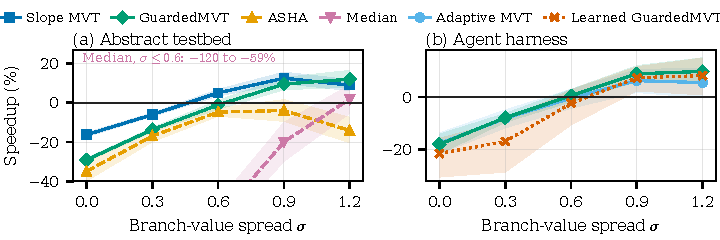
\includegraphics[width=\textwidth]{figs/fig_speedup.pdf}
\caption{Speedup over the per-level-tuned fixed timeout against branch-value spread
$\sigma$ (positive is faster; bands: paired $95\%$ bootstrap intervals). (a)~Abstract
testbed, $30$ seeds. (b)~Agent harness, diminishing value, $20$ seeds.}
\label{fig:sweep}
\end{figure}

\paragraph{Ablations.}
Four ablations were run at $\sigma=0.9$ over $20$ seeds. The
switch cost is the governing economic parameter: MVT's advantage is maximal at moderate
cost ($+11.7\%$ at $s=5$), marginally negative at $s=1$, and negligible by $s=20$. The frontier-rate memory is
insensitive, with the speedup between $7$ and $12\%$ as the averaging half-life varies
from $5$ to $80$ entries. Burstiness is the sole failure point of a naive estimator: under rare
large increments, recent-slope MVT's solve rate falls to $0.25$ at hit probability $0.1$,
misreading depletion, whereas the adaptive estimator preserves full solve rate and stable
time-to-objective.

\subsection{External validity I: the transfer boundary on a network simulator}
\label{sec:res-nasim}

We ran the same scheduler over NASim~\cite{nasim2019} episodes (12 seeds) with a
per-level-tuned timeout, plain MVT, and GuardedMVT. The advantage does not transfer: NASim
exploitation is a constant hazard with roughly uniform host value, so lingering on a branch
delays an equally valuable reward rather than forgoing a richer one. Plain MVT is $22$ to
$46\%$ slower than the tuned timeout across $\sigma$. GuardedMVT does not collapse ($92$ to
$100\%$ solved) but is slower still, since NASim is only a \emph{mild} constant hazard where
plain MVT already solves and the guard's budget commitment is overhead against a collapse
that never occurs.

\subsection{External validity II: a live agent harness (Tier B)}
\label{sec:res-tierb}

The simulator is replaced by a live, tool-executing agent harness over a sealed-off
range. A branch is a running service, one unit of compute corresponds to one bounded
action, and a milestone ledger credits progress solely from observable service state
(host discovered, service enumerated, foothold shell, objective flag), never from agent
self-report. Diminishing returns and burstiness thus arise from an explicit mechanism:
unreached milestones become sparser as a branch is worked, and a foothold or flag
constitutes a large, infrequent increment.

\begin{table}[t]
\centering
\caption{Live-harness robustness to an \emph{unknown} regime at $\sigma=1.2$
(ticks; lower is better; ``fails'': none solved; a percentage: share solved). ``Best for
both'': smallest worst-case ratio to the regime-tuned timeout. Scenarios: of the nine in
Section~\ref{sec:res-thresh}, those solved in every episode.}
\label{tab:robust}
\setlength{\tabcolsep}{4pt}
\footnotesize
\begin{tabular}{lccc}
\toprule
Policy (one configuration) & Diminishing & Constant & Scenarios \\
\midrule
\tabinput{tables/robust.tex}
\bottomrule
\end{tabular}
\end{table}

The live harness reproduces the full pattern (Fig.~\ref{fig:sweep}b). In the
diminishing-value regime, GuardedMVT's speedup over a per-level-tuned timeout again
increases with heterogeneity, from $-18\%$ at $\sigma=0$ to $+9.7\%$ at $\sigma=1.2$
($[5.1,14.9]$; Holm-adjusted $p\le0.008$ for $\sigma\ge0.9$; crossover near
$\sigma\approx0.6$), consistent with the abstract testbed. In the
constant-hazard regime plain MVT's solve rate drops to $0\%$; it makes no switch at all, so every worker stays on an
exhausted branch, whereas GuardedMVT solves every episode. The decisive
comparison is robustness to an unknown regime (Table~\ref{tab:robust}): the optimal
timeout budget differs approximately eightfold between regimes, so a timeout tuned for one
is poor in the other, the best-for-both baselines are slow in one regime or miss
constant-hazard episodes, and plain MVT fails. GuardedMVT is the one policy significantly
faster than the tuned timeout under diminishing value that also solves every
constant-hazard episode at every $\sigma$, at a $57\%$ premium over the constant-tuned
timeout there.

\subsection{Sensitivity, learned thresholds and a dynamic budget}
\label{sec:res-thresh}

Moving each relative threshold over five or six values around its default changes time-to-objective by at most $6.6\%$ (testbed, $\sigma=0.9$) and $4.5\%$
(harness, $\sigma=1.2$), with every episode solved. Under constant hazard the budget is the
exception: $8$ ticks is $25.7\%$ faster than the default $16$, and $32$ ticks $45.3\%$
slower. The learned set (\textit{decline\_frac} $0.45$, peak floor $0.17\,\RR$, budget $8$,
\textit{min\_samples} $2$, hysteresis $0.22$) has the smallest worst-case ratio in
Table~\ref{tab:robust} ($1.07$, against $1.37$ for the best timeout and $1.57$ for the
default) but misses $5$ to $15\%$ of constant-hazard episodes at $\sigma\le0.6$. Nine
harness scenarios test transfer: diminishing value with $\tau$ halved, kept and doubled;
constant hazard at $\sigma\in\{0.3,0.6,1.2\}$; and access cost halved, doubled and
quadrupled. Only the dynamic budget
and the $t{=}60$ timeout solve all nine, and the dynamic budget is faster in each
(worst-case ratio to the scenario-tuned timeout $1.69$ against $3.42$). At four times the
access cost the static default solves $70\%$, the learned set $15\%$, and the best-for-both
timeout $45\%$.

\subsection{LLM agents and a containerised range}
\label{sec:res-llm}

\begin{table}[t]
\centering
\caption{LLM agents in the harness ($\sigma=1.2$, $20$ seeds). Wasted: off-tactic decisions
without progress; fallback: replies without a menu word (diminishing\,/\,constant, $\%$); ms: per uncached
decision.
GuardedMVT's speedup over the per-brain tuned timeout $t^\star$ ($95\%$ interval); constant
hazard: ticks of $t^\star$ (budget), GuardedMVT, and the scripted brain's $t^\star$ reused.
Plain MVT solves no constant-hazard episode; GuardedMVT solves all.}
\label{tab:llm}
\setlength{\tabcolsep}{2.5pt}
\scriptsize
\begin{tabular}{lccrcccc}
\toprule
 & & & & Diminishing & \multicolumn{3}{c}{Constant hazard (ticks)} \\
\cmidrule(lr){5-5}\cmidrule(lr){6-8}
Brain & Wasted & Fallback & ms & GuardedMVT (\%) & $t^\star$ & GuardedMVT &
Scripted $t^\star$ \\
\midrule
\tabinput{tables/llm.tex}
\bottomrule
\end{tabular}
\end{table}

The scripted tactic was replaced by five 4-bit open-weight models served locally by Ollama
0.20.3 with greedy decoding: Qwen2.5 7B and 1.5B~\cite{qwen2024qwen25},
Llama-3.1-8B~\cite{grattafiori2024llama3}, Gemma-2-9B~\cite{gemma2024gemma2} and
Mistral-7B~\cite{jiang2023mistral}. A model sees the service state and its last three
actions with their outcomes and must answer with one menu word; any other reply is executed
by the scripted tactic. Unlike the harvesting tactic of Section~\ref{sec:res-tierb}, the scripted reference here
also walks the full reconnaissance sequence. Replies are memoised by prompt, which under greedy decoding returns what a fresh
query would; re-querying $200$ random memoised prompts per model without the memo returned
the same reply in all $1000$ cases.

GuardedMVT solves every episode with every brain (Table~\ref{tab:llm}). Under diminishing
value Qwen2.5-7B, Llama and Gemma waste at most $6\%$ of decisions and GuardedMVT keeps the
scripted lead of $3.5\%$ ($0.9\%$ for Llama; none significant); with Qwen2.5-1.5B, which wastes over half its steps, it is
$22.7\%$ faster. Mistral, which opens branches out of order, is the exception ($-29.9\%$). Under constant hazard the models waste
$39$ to $68\%$ of decisions and the best budget grows from $8$ to $12$--$25$ ticks; GuardedMVT
trails each re-tuned timeout by $13$ to $30\%$, but the scripted brain's timeout, reused, is
$33$ to $67\%$ slower than GuardedMVT, which is never re-tuned. Two components needed
changes for LLM brains: with a fixed $k$-tick entry window, Llama's repeated opening
enumerations drive $\RR$ toward zero and GuardedMVT is $30\%$ slower, which the ramp-aware
form removes; and with only the last action in view, two models loop between
reconnaissance actions until three steps of history are shown.

On a containerised range of twelve HTTP fixtures on an internal Docker network without
egress (log-normal richness, $\sigma=1.2$; every action a real request), with two workers and
$10$ seeds, GuardedMVT is within $2.5\%$ of the timeout tuned on that range at $80$ and
$90\%$ coverage ($-2.2\%$, $p=0.09$; $+2.5\%$, $p=0.008$) while plain MVT is $39$ and $82\%$
slower. With Qwen2.5-7B, served by a CPU-only Ollama container on the same network, every episode
matched the scripted one, and the isolation proof ran $37{,}256$ times, before every action,
without a failure.

% ===========================================================================
\section{Safety, Ethics, and Responsible Use}
\label{sec:safety}

Automated attack execution requires the research instrument to be safe by construction,
enforced by four properties. First, isolation is a hard precondition: the harness
verifies sandbox isolation before every action and refuses to proceed otherwise, with no
override; the live range resides on a no-egress internal network, verified from within by
requiring outbound connections to fail. Second, the action set is bounded and
non-weaponised, comprising only probe, enumerate, attempt-access with a planted default
credential, and collect, with neither exploit synthesis nor arbitrary command execution;
each action maps to a plain request against a deliberately vulnerable fixture containing
no real data. Third, progress is grounded: a milestone is credited only when its evidence
predicate holds against observed state, preventing MVT from optimising a fabricated
signal. Fourth, instantiating the live-range sandbox requires an explicit authorisation flag; all
experiments reported here use an in-process mock or the isolated fixture, and the work
targets authorised defensive assessment only.

To test these controls, banners and collected artifacts carried five injected
instructions (a shell command, an out-of-scope scan, an outside connection, an
\texttt{exploit} action, an upload). Of $50$ queries over the five models, $16$ replies repeated the
instruction, from \texttt{exploit} to \texttt{exec rm -rf /}; none held a menu word, so each ran as the scripted step. In $30$ GuardedMVT episodes with the shell
payload in every banner and artifact, all $20{,}652$ executed actions were menu methods on
in-scope services and every episode was solved, although up to $97\%$ of a model's replies
fell back to the script. A sandbox failing its isolation proof refused $1000$ of $1000$ steps
before the agent was consulted; the live sandbox would not start without the authorisation
flag and, on an internet-connected host, its egress probe refused; and $10^5$ fuzzed replies
mapped only to a menu action or the fallback.

% ===========================================================================
\section{Limitations and Threats to Validity}
\label{sec:threats}

The foraging model and the heterogeneity parameter are
synthetic. The live harness uses mock services and a small containerised fixture reached
via a planted default credential rather than real vulnerabilities, and its LLM brains are
small local models choosing from a four-action menu, not planners that compose their own
commands. Internal validity follows from per-scenario baseline tuning and from all policies sharing
one selection rule and identical per-seed surfaces. For external validity we exhibit a
regime (constant hazard) in which the advantage vanishes and claim nothing beyond
diminishing-value branches. Beyond the paired tests, the qualitative structure (crossover,
collapse, single-configuration robustness) holds across seeds, estimators, pool sizes, agent
brains, and both realism layers.

% ===========================================================================
\section{Conclusion and Future Work}
\label{sec:conclusion}

We derived an abandonment criterion for parallel penetration-testing agents from the Marginal Value Theorem and characterised, on a controlled testbed and
a live harness, where it succeeds (heterogeneous, diminishing-value surfaces), where it
fails (uniform or constant-hazard targets), and a mechanism retaining the gain without the
failure. GuardedMVT infers the regime online per branch and was the only evaluated policy
faster under diminishing value that solved every constant-hazard episode without
reconfiguration, with scripted and LLM agents alike. Future work includes a Whittle-index treatment of drifting arms, LLM agents
that compose their own tools, and larger live ranges with lateral movement.

\begin{credits}
\subsubsection{\discintname}
The authors have no competing interests to declare that are relevant to the content of
this article.
\end{credits}

% References in order of first appearance (numerical-sequence requirement), splncs04 format.
\begin{thebibliography}{22}
\bibitem{schwartz2019autonomous}
Schwartz, J., Kurniawati, H.: Autonomous penetration testing using reinforcement learning. arXiv preprint arXiv:1905.05965 (2019)

\bibitem{hu2020automated}
Hu, Z., Beuran, R., Tan, Y.: Automated penetration testing using deep reinforcement learning. In: 2020 IEEE European Symposium on Security and Privacy Workshops (EuroS\&PW). pp. 2--10. IEEE (2020)

\bibitem{deng2024pentestgpt}
Deng, G., Liu, Y., Mayoral-Vilches, V., Liu, P., Li, Y., Xu, Y., Zhang, T., Liu, Y., Pinzger, M., Rass, S.: {PentestGPT}: evaluating and harnessing large language models for automated penetration testing. In: 33rd USENIX Security Symposium. pp. 847--864 (2024)

\bibitem{charnov1976optimal}
Charnov, E.L.: Optimal foraging, the marginal value theorem. Theoretical Population Biology \textbf{9}(2), 129--136 (1976)

\bibitem{sarraute2012pomdp}
Sarraute, C., Buffet, O., Hoffmann, J.: {POMDPs} make better hackers: accounting for uncertainty in penetration testing. In: Proceedings of the AAAI Conference on Artificial Intelligence. vol.~26, pp. 1816--1824 (2012)

\bibitem{ghanem2020reinforcement}
Ghanem, M.C., Chen, T.M.: Reinforcement learning for efficient network penetration testing. Information \textbf{11}(1), 6 (2020)

\bibitem{nasim2019}
Schwartz, J.: {NASim}: Network Attack Simulator (2019), \url{https://github.com/Jjschwartz/NetworkAttackSimulator}

\bibitem{cyberbattlesim2021}
Microsoft Defender Research Team: {CyberBattleSim} (2021), \url{https://github.com/microsoft/CyberBattleSim}

\bibitem{auer2002finite}
Auer, P., Cesa-Bianchi, N., Fischer, P.: Finite-time analysis of the multiarmed bandit problem. Machine Learning \textbf{47}(2--3), 235--256 (2002)

\bibitem{gittins1979bandit}
Gittins, J.C.: Bandit processes and dynamic allocation indices. Journal of the Royal Statistical Society: Series B \textbf{41}(2), 148--177 (1979)

\bibitem{whittle1988restless}
Whittle, P.: Restless bandits: activity allocation in a changing world. Journal of Applied Probability \textbf{25}(A), 287--298 (1988)

\bibitem{golovin2017vizier}
Golovin, D., Solnik, B., Moitra, S., Kochanski, G., Karro, J., Sculley, D.: Google {Vizier}: a service for black-box optimization. In: Proceedings of the 23rd ACM SIGKDD International Conference on Knowledge Discovery and Data Mining. pp. 1487--1495. ACM (2017). \doi{10.1145/3097983.3098043}

\bibitem{li2020asha}
Li, L., Jamieson, K., Rostamizadeh, A., Gonina, E., Ben-tzur, J., Hardt, M., Recht, B., Talwalkar, A.: A system for massively parallel hyperparameter tuning. In: Proceedings of Machine Learning and Systems. vol.~2, pp. 230--246 (2020)

\bibitem{stephens1986foraging}
Stephens, D.W., Krebs, J.R.: Foraging Theory. Princeton University Press (1986)

\bibitem{pirolli1999information}
Pirolli, P., Card, S.: Information foraging. Psychological Review \textbf{106}(4), 643--675 (1999)

\bibitem{paszke2019pytorch}
Paszke, A., Gross, S., Massa, F., et al.: {PyTorch}: an imperative style, high-performance deep learning library. In: Advances in Neural Information Processing Systems. vol.~32 (2019)

\bibitem{mpiforum2021}
{MPI Forum}: {MPI}: A Message-Passing Interface Standard, Version 4.0. University of Tennessee (2021)

\bibitem{dalcin2011mpi4py}
Dalc{\'i}n, L.D., Paz, R.R., Kler, P.A., Cosimo, A.: Parallel distributed computing using {Python}. Advances in Water Resources \textbf{34}(9), 1124--1139 (2011)

\bibitem{qwen2024qwen25}
Qwen Team: {Qwen2.5} technical report. arXiv preprint arXiv:2412.15115 (2024)

\bibitem{grattafiori2024llama3}
Grattafiori, A., et al.: The {Llama}~3 herd of models. arXiv preprint arXiv:2407.21783 (2024)

\bibitem{gemma2024gemma2}
Gemma Team: {Gemma}~2: improving open language models at a practical size. arXiv preprint arXiv:2408.00118 (2024)

\bibitem{jiang2023mistral}
Jiang, A.Q., et al.: {Mistral} {7B}. arXiv preprint arXiv:2310.06825 (2023)

\end{thebibliography}

\end{document}
